\documentclass[border=4pt,12pt]{standalone}
% House style for redrawn exam diagrams (diagram-v4: 0.4pt lines, filled -latex arrows, fine dashes; stipple and hatching drawn as real dots/lines (no PDF/SVG patterns, so they render in every browser and at any scale); transparent background). Every figure \input's this.
\usepackage{amsmath,amssymb}
\usepackage{txfonts}
\usepackage{pdfrender,xcolor}
% \halo{text}: label on shading. The shading stops just around each letter's outline (a thin knock-out that follows the
% glyphs, like the papers' typesetting), never a box. Owner: "I don't want a box around the text".
\newcommand{\halo}[1]{\leavevmode\rlap{\pdfrender{TextRenderingMode=2,LineWidth=2.2pt,LineJoinStyle=1,StrokeColor=white,FillColor=white}#1}#1}
\usepackage{tikz,pgfplots}
\pgfplotsset{compat=1.18}
\usetikzlibrary{arrows.meta,calc,angles,quotes,patterns,patterns.meta,intersections,positioning,decorations.markings,shapes.geometric}
% Stipple and hatching are drawn as actual dots / lines clipped to the region (path picture), NOT as pattern fills:
% SVG <pattern> fills vanish or blur when browsers scale the image, so the owner could not see the shading.
% Each dot is a 0.72pt square (keeps SVGs small; reads as a dot at print size). Dots sit on one global staggered grid, so neighbouring regions line up.
\makeatletter
\newdimen\ex@x \newdimen\ex@y \newdimen\ex@xa \newdimen\ex@ya \newdimen\ex@xb \newdimen\ex@yb \newcount\ex@row
\def\exam@stipplecolor{black!75}\def\exam@dotr{0.42pt}\def\exam@dotgap{2.5}
\def\ex@rowdots{\ifdim\ex@x<\ex@xb \pgfpathrectangle{\pgfqpoint{\dimexpr\ex@x-0.36pt\relax}{\dimexpr\ex@y-0.36pt\relax}}{\pgfqpoint{0.72pt}{0.72pt}}\advance\ex@x by \exam@dotgap pt\relax\expandafter\ex@rowdots\fi}
\def\exam@stipple{%
  \pgftransformreset% dots are sized in real points even inside scaled pictures
  \pgfpointanchor{path picture bounding box}{south west}\ex@xa=\pgf@x \ex@ya=\pgf@y
  \pgfpointanchor{path picture bounding box}{north east}\ex@xb=\pgf@x \ex@yb=\pgf@y
  \pgfsetfillcolor{\exam@stipplecolor}\pgfmathsetmacro\ex@h{\exam@dotgap/2}%
  \pgfmathtruncatemacro\ex@r{floor(\ex@ya/\ex@h)-1}\ex@row=\ex@r\relax
  \ex@y=\ex@r\dimexpr\ex@h pt\relax
  \loop\ifdim\ex@y<\ex@yb
    \pgfmathtruncatemacro\ex@c{floor(\ex@xa/\exam@dotgap)-1}\ex@x=\ex@c\dimexpr\exam@dotgap pt\relax
    \ifodd\ex@row \advance\ex@x by \ex@h pt\fi
    \ex@rowdots
    \advance\ex@y by \ex@h pt \advance\ex@row by 1
    \ifnum\numexpr\ex@row-(\ex@row/4)*4\relax=0 \pgfusepath{fill}\fi% flush every 4 rows: bounded TeX memory, few clip copies in the SVG
  \repeat\pgfusepath{fill}}
\newdimen\ex@d
\def\exam@hatch#1{% #1 = 1 for /, -1 for \ ; lines 45 degrees, 3pt apart
  \pgftransformreset
  \pgfpointanchor{path picture bounding box}{south west}\ex@xa=\pgf@x \ex@ya=\pgf@y
  \pgfpointanchor{path picture bounding box}{north east}\ex@xb=\pgf@x \ex@yb=\pgf@y
  \ex@d=\dimexpr\ex@yb-\ex@ya\relax \ex@x=\dimexpr\ex@xa-\ex@d\relax
  \loop\ifdim\ex@x<\ex@xb
    \ifnum#1>0 \pgfpathmoveto{\pgfqpoint{\ex@x}{\ex@ya}}\pgfpathlineto{\pgfqpoint{\dimexpr\ex@x+\ex@d\relax}{\ex@yb}}%
    \else \pgfpathmoveto{\pgfqpoint{\ex@x}{\ex@yb}}\pgfpathlineto{\pgfqpoint{\dimexpr\ex@x+\ex@d\relax}{\ex@ya}}\fi
    \advance\ex@x by 4.24pt
  \repeat
  \pgfsetlinewidth{0.4pt}\pgfsetstrokecolor{black}\pgfusepath{stroke}}
\def\examstipple{\exam@stipple}\def\examhatch{\exam@hatch}\def\examsetstipplecolor#1{\def\exam@stipplecolor{#1}}\def\examsetdotgap#1{\def\exam@dotgap{#1}}
\makeatother
% (legacy pattern kept for old files)
% staggered stipple like the NESA papers' dotted shading
\pgfdeclarepatternformonly{exam stipple}{\pgfpointorigin}{\pgfqpoint{2.2pt}{2.2pt}}{\pgfqpoint{2.2pt}{2.2pt}}{%
  \pgfpathcircle{\pgfqpoint{0.55pt}{0.55pt}}{0.42pt}\pgfpathcircle{\pgfqpoint{1.65pt}{1.65pt}}{0.42pt}\pgfusepath{fill}}
\tikzset{
  every picture/.style={line width=0.6pt, >={Latex[length=2mm,width=1.3mm]}},
  curve/.style={line width=0.6pt},
  open arrow/.style={-{Latex[length=2mm,width=1.3mm]}},  % owner: filled -latex heads everywhere, no open chevrons
  aux/.style={dash pattern=on 2pt off 1.5pt, line width=0.6pt},
  shade/.code={\def\exA{#1}\def\exB{none}\ifx\exA\exB\else\pgfkeysalso{fill=black!18}\fi},
  shade/.default=on,
  shade dots/.style={fill=none, path picture={\examstipple}},
  stipple color/.code={\examsetstipplecolor{#1}},
  stipple gap/.code={\examsetdotgap{#1}},
  shade dense dots/.style={fill=none, stipple gap=1.6, path picture={\examstipple}},
  shade hatch/.style={fill=none, path picture={\examhatch{1}}},
  shade hatch reverse/.style={fill=none, path picture={\examhatch{-1}}},
  shade solid/.style={fill=black},
  pt/.style={circle, fill, inner sep=1.1pt},
  open pt/.style={circle, draw, fill=white, inner sep=1.1pt},
}
\pgfplotsset{
  exam axes/.style={axis lines=middle, axis line style={->}, xlabel={$x$}, ylabel={$y$},
    xlabel style={anchor=west}, ylabel style={anchor=south}, tick label style={font=\small},
    every axis plot/.append style={line width=0.6pt, black}, samples=200, clip=false,
    enlargelimits=false, axis on top},
}

\begin{document}
% 571_q20_s1: solution screenshot: the question graph of y=f'(x) (dashed, scaled 1.012) with the sketch of y=f(x); clipped to the crop window as the screenshot is
% y=f'(x) is a sketch (not a polynomial): traced from 571_q20_1 and refitted smooth, pinned to f'(0)=2, the touch at (1,0),
% the root at 3 and the max at x=2, y=2.5 on the paper's grid (rule 16). The curve starts just right of the tick label 3 (rule 11).
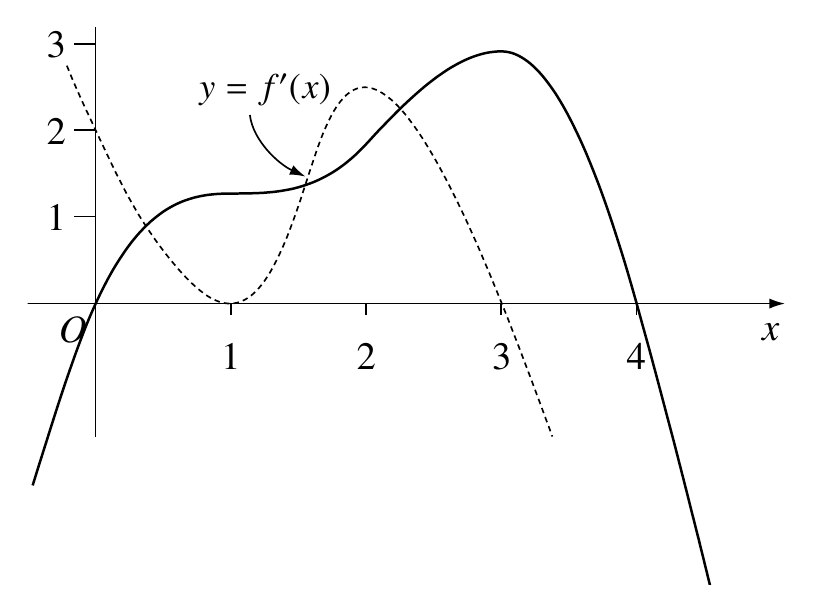
\begin{tikzpicture}[x=0.0127cm,y=-0.0127cm, every node/.style={font=\fontsize{14}{17}\selectfont}]
  \begin{scope}
  \clip (0,20) rectangle (779,577);
  \draw[->] (-67.1,296.0) -- (757.7,296.0);
  \draw[->] (68.0,429.1) -- (68.0,-44.5);
  \draw (203.1,296.0) -- (203.1,307.6);
  \draw (338.4,296.0) -- (338.4,307.6);
  \draw (473.7,296.0) -- (473.7,307.6);
  \draw (608.9,296.0) -- (608.9,307.6);
  \draw (46.2,36.4) -- (68.0,36.4);
  \draw (46.2,122.4) -- (68.0,122.4);
  \draw (46.2,209.0) -- (68.0,209.0);
  \draw[aux] plot[smooth] coordinates {(39.2,58.0) (45.1,72.4) (51.1,86.0) (57.0,99.1) (63.0,111.8) (68.9,124.5) (74.9,137.2) (80.9,149.8) (86.8,162.2) (92.8,174.1) (98.7,185.5) (104.7,196.2) (110.6,206.4) (116.6,215.9) (122.6,224.9) (128.5,233.4) (134.5,241.5) (140.4,249.1) (146.4,256.4) (152.3,263.3) (158.3,269.8) (164.2,275.7) (170.2,281.1) (176.2,285.8) (182.1,289.8) (188.1,292.8) (194.0,294.9) (200.0,295.9) (205.9,295.8) (211.9,294.5) (217.9,291.8) (223.8,287.8) (229.8,282.2) (235.7,275.0) (241.7,266.1) (247.6,255.4) (253.6,243.0) (259.6,229.0) (265.5,213.4) (271.5,196.4) (277.4,178.3) (283.4,160.0) (289.3,142.3) (295.3,126.3) (301.3,112.8) (307.2,101.9) (313.2,93.4) (319.1,87.1) (325.1,82.8) (331.0,80.4) (337.0,79.6) (343.0,80.3) (348.9,82.3) (354.9,85.5) (360.8,89.7) (366.8,94.8) (372.7,100.9) (378.7,107.9) (384.6,115.7) (390.6,124.1) (396.6,133.2) (402.5,143.0) (408.5,153.2) (414.4,164.0) (420.4,175.3) (426.3,187.0) (432.3,199.2) (438.3,211.8) (444.2,224.8) (450.2,238.2) (456.1,252.0) (462.1,266.1) (468.0,280.5) (474.0,295.2) (480.0,310.1) (485.9,325.3) (491.9,340.7) (497.8,356.3) (503.8,372.1) (509.7,388.0) (512.8,396.2) (515.8,404.4) (518.8,412.6) (521.9,420.8) (524.9,429.1)};
  \draw[->] (222.3,107.3) .. controls (225.4,133.6) and (251.7,156.8) .. (278.0,169.0);
  \node[anchor=center, inner sep=0pt] at (742.5,324.8) {$x$};
  \node[anchor=center, inner sep=0pt] at (50.3,-33.4) {$y$};
  \node[anchor=center, inner sep=0pt] at (45.2,322.8) {$O$};
  \node[anchor=center, inner sep=0pt] at (203.1,349.1) {$1$};
  \node[anchor=center, inner sep=0pt] at (338.7,349.1) {$2$};
  \node[anchor=center, inner sep=0pt] at (474.3,349.1) {$3$};
  \node[anchor=center, inner sep=0pt] at (608.9,349.1) {$4$};
  \node[anchor=east, inner sep=0pt] at (39.2,37.4) {$3$};
  \node[anchor=east, inner sep=0pt] at (39.2,123.5) {$2$};
  \node[anchor=east, inner sep=0pt] at (39.2,209.5) {$1$};
  \node[font=\fontsize{13}{16}\selectfont] at (237.5,82.0) {$y=f'(x)$};
  % y=f(x) (teacher sketch, redrawn clean, black): through O, horizontal point of inflection at x=1, max at x=3 (rule 18),
  % crossing the x-axis at 4 and the heights as sketched; the teacher's circle at x=1, tick at the max and cut-off pen marks
  % at the top edge are left out (rule 17).
  \draw[line width=0.9pt] plot[smooth] coordinates {(5.0,477.9) (11.2,457.9) (17.5,438.0) (23.7,418.3) (29.9,398.9) (36.1,380.0) (42.4,361.7) (48.6,344.2) (54.8,327.6) (61.0,312.0) (67.3,297.6) (73.5,284.5) (79.7,272.4) (85.9,261.3) (92.2,251.2) (98.4,242.0) (104.6,233.7) (110.8,226.3) (117.1,219.6) (123.3,213.7) (129.5,208.6) (135.7,204.0) (142.0,200.1) (148.2,196.8) (154.4,194.0) (160.6,191.8) (166.9,189.9) (173.1,188.5) (179.3,187.4) (185.5,186.7) (191.8,186.2) (198.0,186.0) (204.2,185.9) (210.5,185.9) (216.7,185.8) (222.9,185.7) (229.1,185.5) (235.4,185.2) (241.6,184.7) (247.8,184.1) (254.0,183.2) (260.3,182.1) (266.5,180.8) (272.7,179.1) (278.9,177.1) (285.2,174.8) (291.4,172.1) (297.6,169.0) (303.8,165.5) (310.1,161.5) (316.3,157.0) (322.5,152.0) (328.7,146.5) (335.0,140.3) (341.2,133.7) (347.4,126.9) (353.6,120.3) (359.9,113.9) (366.1,107.5) (372.3,101.3) (378.5,95.4) (384.8,89.6) (391.0,84.1) (397.2,78.8) (403.5,73.8) (409.7,69.1) (415.9,64.8) (422.1,60.7) (428.4,57.1) (434.6,53.8) (440.8,51.0) (447.0,48.6) (453.3,46.6) (459.5,45.1) (465.7,44.2) (471.9,43.7) (478.2,44.0) (484.4,45.3) (490.6,47.8) (496.8,51.4) (503.1,56.1) (509.3,61.9) (515.5,68.8) (521.7,76.8) (528.0,85.8) (534.2,95.9) (540.4,107.0) (546.6,119.2) (552.9,132.4) (559.1,146.5) (565.3,161.7) (571.6,177.9) (577.8,195.0) (584.0,213.1) (590.2,232.2) (596.5,252.2) (602.7,273.1) (608.9,294.9) (615.1,317.4) (621.4,340.1) (627.6,363.1) (633.8,386.4) (640.0,409.9) (646.3,433.7) (652.5,457.8) (658.7,482.1) (664.9,506.7) (671.2,531.6) (677.4,556.7) (683.6,582.1)};
  \end{scope}
\end{tikzpicture}
\end{document}
